\subsection{Assignment 2. Finite Element Method}
\subsubsection{Derive quadratic interpolation functions for the finite element method. Plot them in local coordinates. Show your derivation.}
As shown in the lecture, for the square shape functions, we can write our trial solution as:
\begin{align}
\widehat{T} &= a_0 + a_1 x +a_2 x^{2}\\
     &= \underbrace{\begin{bmatrix}1 & x & x^2\end{bmatrix}}_{X} \underbrace{\begin{bmatrix}a_0 & a_1 & a_2\end{bmatrix}^T}_{A}\\
    T_{i_{1}} &= T(0) = a_0 + a_1 \cdot 0 + a_2 \cdot 0^2\\
    T_{i_{2}} &= T(1/2) = a_0 + \frac{a_1}{2} + \frac{a_2}{2^2}\\
    T_{i_{3}} &= T(1) = a_0 + a_1 \cdot 1+a_2 \cdot 1^2  \\
    \underbrace{\begin{bmatrix}T_{i_1} \\ T_{i_2} \\ T_{i_3}\end{bmatrix}}_{T} &=
         \underbrace{\begin{bmatrix}
         1 & 0 & 0\\
         1 & \frac{1}{2} & \frac{1}{2^2}\\
         1 & 1 & 1\end{bmatrix}}_{L}
         \underbrace{\begin{bmatrix}a_0 \\ a_1 \\ a_2\end{bmatrix}}_{A} \\
         XA &= NLA\\
         N &= XL^{-1}\\
         &= \begin{bmatrix} 2\,x^2-3\,x+1 & 4\,x-4\,x^2 & 2\,x^2-x \end{bmatrix}
\end{align}
\begin{figure}[htb!]
    \centering
    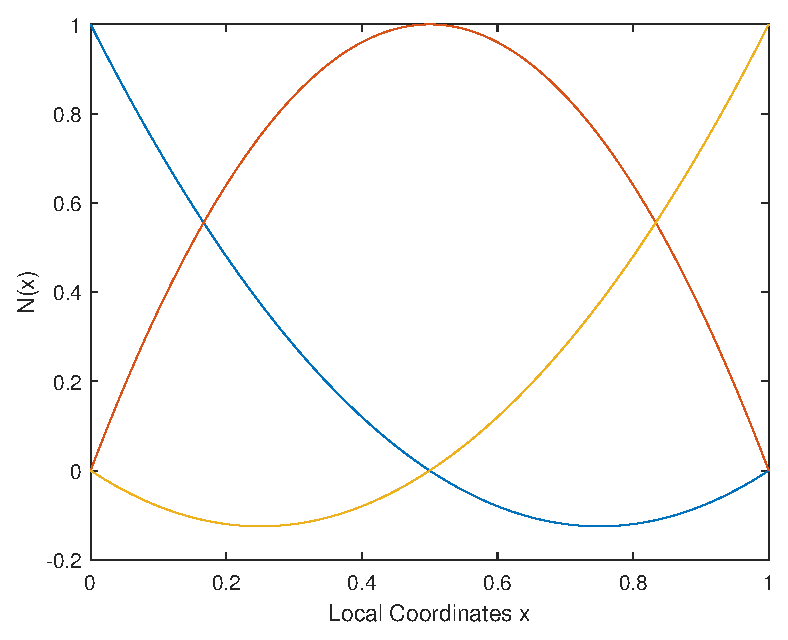
\includegraphics[width=.7\linewidth]{./homework2/img/3.eps}
    \caption{Quadratic FEM Interpolation Functions}
    \label{fig:interpol_functions}
\end{figure}

\subsubsection{ Consider a 1D steady state heat conduction problem, where $k$ and $S$ are constant. How would the stiffness matrix for one element look like for the shape functions derived in step 1?}
Problem:
\begin{align}
    kT'' + S &= 0\ \mathrm{on}\ \Omega \in [0,1]\\
    T(0) = &0,\ T(1) = 0 \\
    k_{stiff}(i,j) &= \int_{0}^{1}{N'(i) \cdot N'(j) dx}\\
    k_{stiff} &= \begin{bmatrix}
    2.\bar{3} & -2.\bar{6} &  0.\bar{3} \\
    -2.\bar{6} &  5.\bar{3} & -2.\bar{6} \\
    0.\bar{3} & -2.\bar{6} &  2.\bar{3}\end{bmatrix}
\end{align}
\begin{lstlisting}
%% 3D Finite Element Method

% Local x
x_local = 0:0.01:1;
L = [1,0,0; 1,0.5,0.25;1,1,1];
L_inv = inv(sym(L));

syms x
X = [1,x,x^2];
N = X*L_inv;

figure; %visualize cubic shape functions
for i = 1:length(N)
    plot(x_local, subs(N(i),x_local),'DisplayName',['Square Shape Function ' num2str(i)]); hold on;
end
xlabel('Local Coordinates x');
ylabel('N(x)');
%% Stiffness Matrix
k_stiff = zeros(length(N));

for i = 1:length(N)
    for j = 1:length(N)
        k_stiff(i,j) = double(int( diff(N(i), x).*diff(N(j), x), x, 0, 1 ));
    end
end

nodes = 3; % number of elements
Ke = double(k_stiff);
RHSe = int(N, x, 0, 1)';


L = 1; % domain length
k = 1; %for k = [100,10,1,0.1] %; % thermal conductivity,1
S = 10; %    for S = [100,10,1,0.1]% % source,100
l = L/nodes; % node spacing assuming equidistant nodes
dim = nodes*(nodes - 1) +1; %dimension of stiffness matrix
K = zeros(dim); %initialize stiffness matrix with zeros
RHS = zeros([dim, 1]); %initialize load vector with zeros

for i = 1:nodes %cycle through elements
    
    %compute indices of entries for a given element
    ind_start = 1+(i-1)*(nodes-1);
    ind_end = ind_start + (nodes-1);
    
    % update stiffness matrix with the stiffness matrix of a single element
    K(ind_start:ind_end, ind_start:ind_end) = K(ind_start:ind_end, ...
        ind_start:ind_end) + Ke;
    
    %update load vector
    RHS(ind_start:ind_end) = RHS(ind_start:ind_end)+RHSe;
    
end

K = (k/l)*K; %multiply by constants
F = S*l*RHS;
large_number = 1e6; %a trick not to exclude T(0)
K(1,1) = K(1,1)+large_number;
T_FEM = linsolve(K, F)% solve for T
%
x_coord_FEM = 0:l/(nodes-1):1; %coordinates of nodes
figure;
plot(x_coord_FEM, T_FEM,'k--','DisplayName',['FEM, S=',num2str(S),' k=',...
    num2str(k)]); hold on %plot FEM solution
x_coord_solution = 0:0.01:1; %a grid to compute direct solution on
solution = -S/(2*k)*x_coord_solution.^2+S/k*x_coord_solution; %values of the direct
plot(x_coord_solution, solution,'DisplayName', ['Solution, S=',num2str(S),' k=',...
    num2str(k)]); hold on %visualize the direct solution
xlabel('x');
ylabel('T(x)');
legend({},'Location','northwest');
\end{lstlisting}

\begin{figure}[htb!]
    \centering
    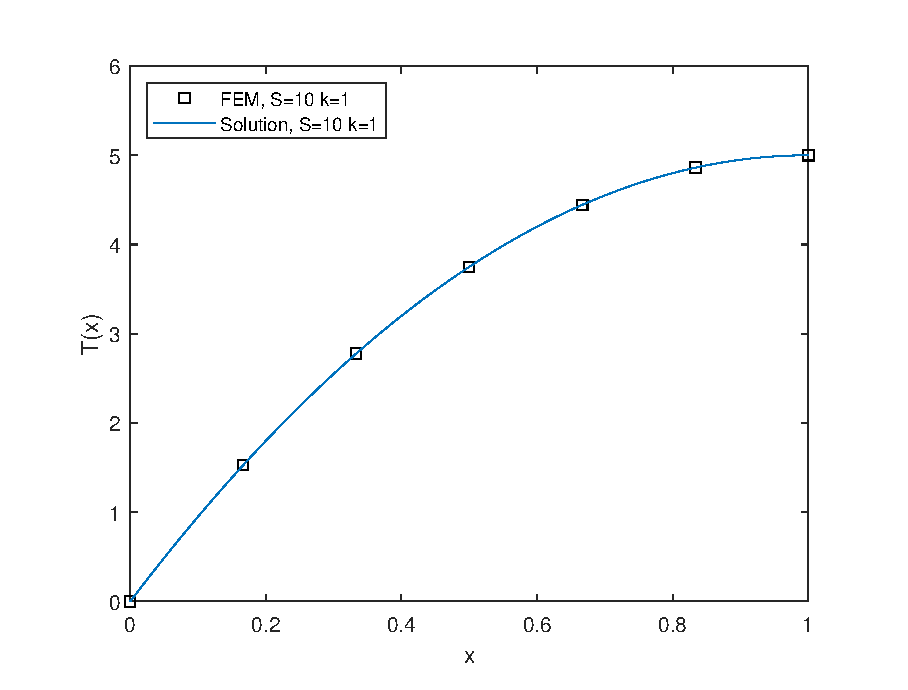
\includegraphics{./homework2/img/final_FEM.eps}
    \caption{Analytical Solution and FEM Approximation}
    \label{fig:sol_FEM}
\end{figure}
%\begin{figure}[htb!]
%    \centering
%    \includegraphics{./homework2/img/5.eps}
%    \caption{Absolute Error of the FEM}
%    \label{fig:error}
%\end{figure}